%!TEX root = TIHSC_Project_main.tex
\chapter{SystemC BCAM}
In the Bus Cycle Accurate Model (BCAM) memory is considered together with the rest of the TLM. 

Now the model is expanded with a memory module, see figure \ref{fig:BCAM}, which contain all the images -- the input image, the filters, the fifteen filtered images and the resulting image. This is approximately 6650 KB data.

\begin{figure}[H]
\centering
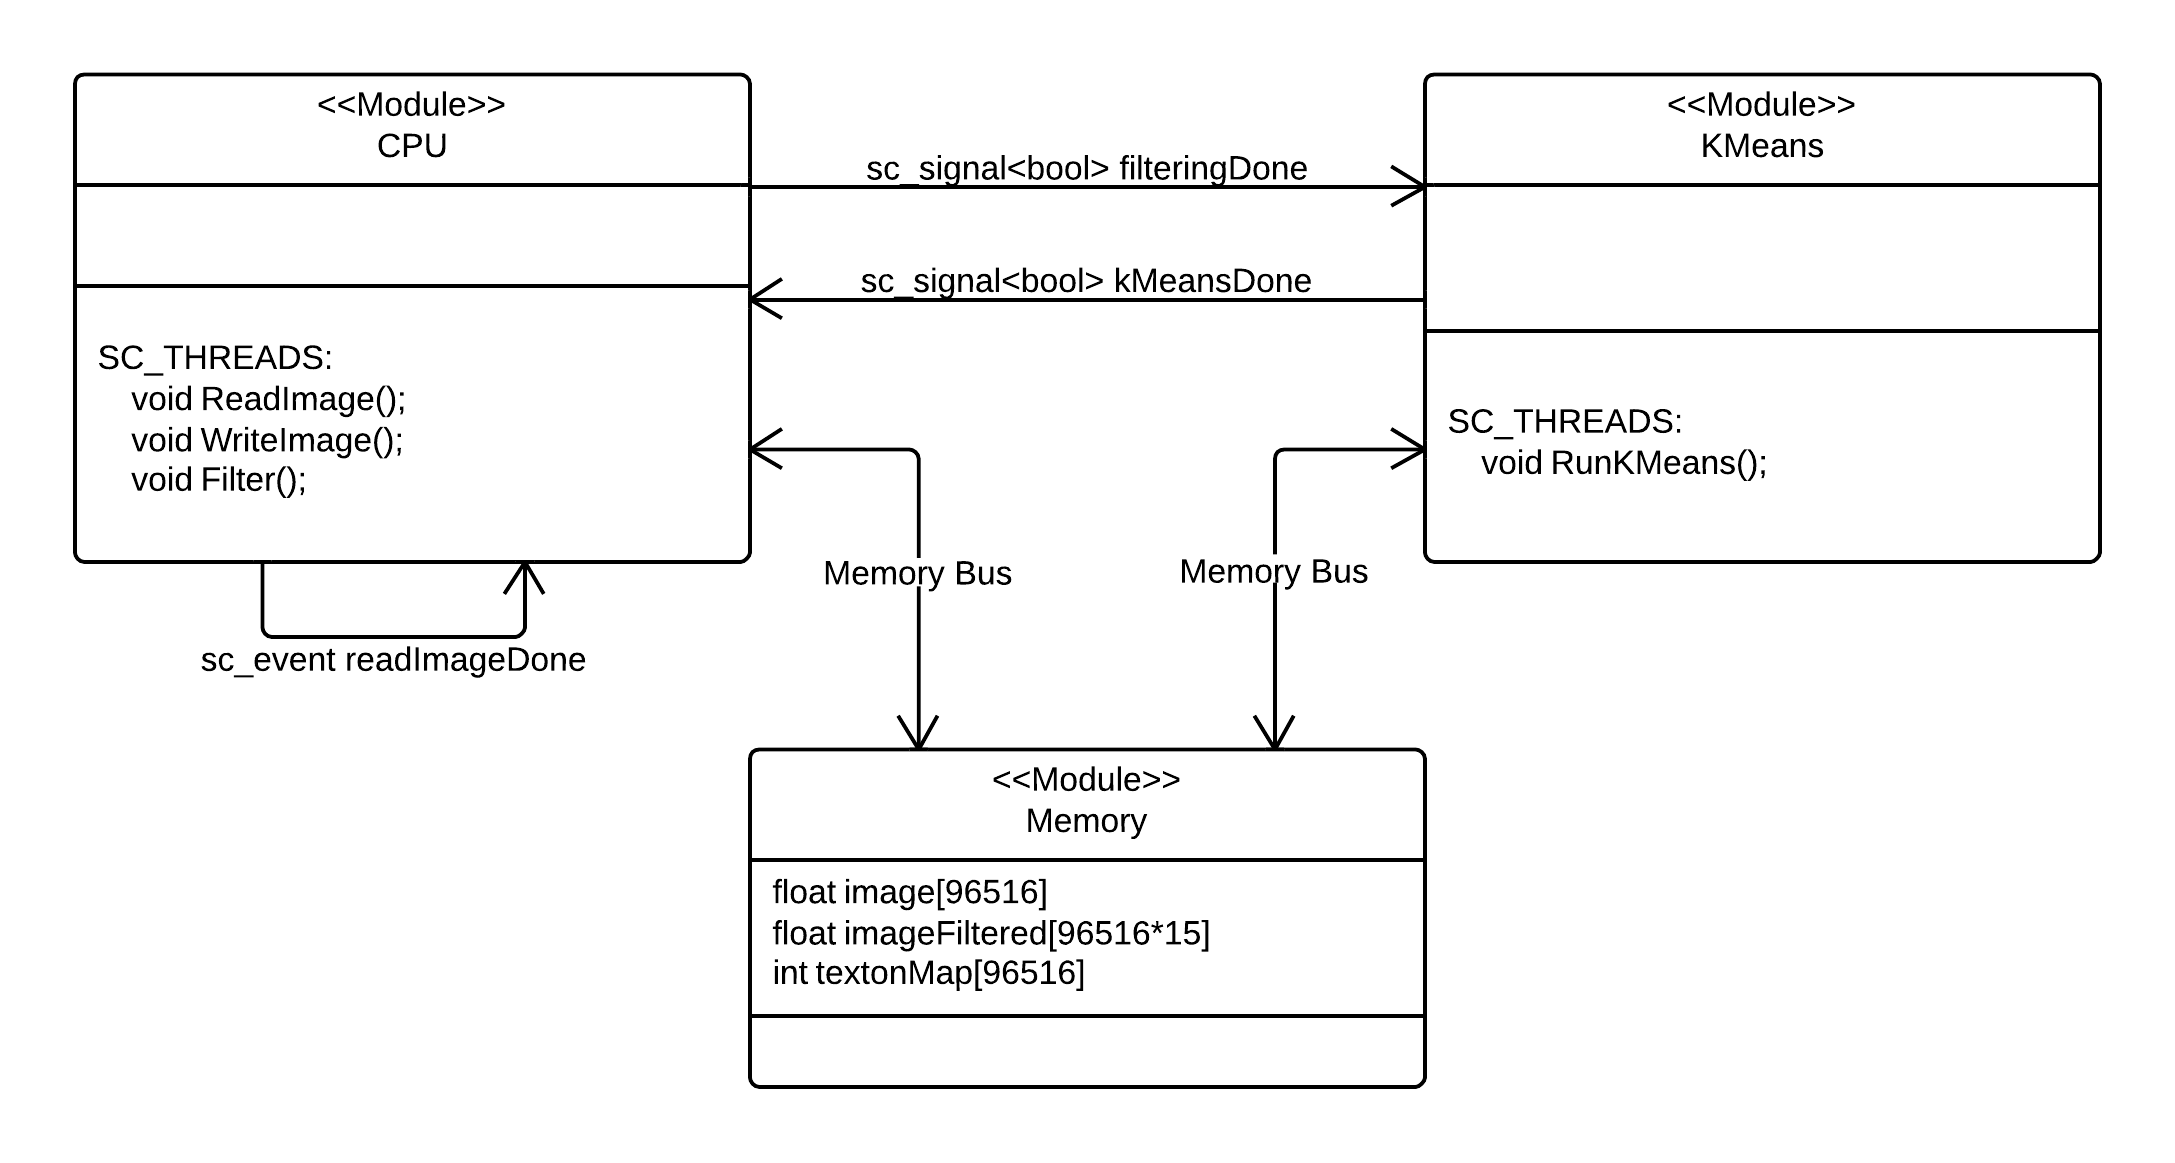
\includegraphics[width = \linewidth]{SystemCBCAM}
\caption{SystemC BCAM diagram}
\label{fig:BCAM}
\end{figure}

\noindent In figure \ref{fig:BCAM} the ``Memory Bus'' represents a memory controller and the connecting busses.

If the k-means module is allocated in hardware communication is handled via busses instead of pointers because hardware and software can not access memory the same way. Hardware components need to be connected to busses, that transfer data to and from the component.

At the Altera DE2 board only 512 KB SRAM memory is available. 
On the contrary it also has 8 MB SDRAM, which demands another memory controller. 
This is a very important consideration in deciding the platform and mapping.


